\rhead{COMMUNICATION}

\lettrine[lines=2,slope=0pt,nindent=4pt]{\textbf{P}}{lusieurs} canaux de communications ont \'et\'e mis en place progressivement autour de TrioCFD
afin de permettre aux utilisateurs et d\'eveloppeurs de TrioCFD d'\'echanger sur le code, sur les difficult\'es qu'ils rencontrent, d'exprimer
leurs besoins autant en terme de d\'eveloppements que d'outils, mais \'egalement de les informer sur les capacit\'es et \'evolutions de
TrioCFD. Chaque canal est d\'edi\'e \`a un type d'information particulier avec une description de chacun d'eux ci-dessous.

\chapter{\label{chapitre:site}Site TrioCFD}
\lhead{Site TrioCFD}
\rhead{COMMUNICATION}

Le site TrioCFD a \'et\'e construit en 2019 et est accessible \`a l'adresse suivante :
"\url{http://triocfd.cea.fr/Pages/Presentation/TrioCFD_code.aspx}". Il est actuellement construit comme illustr\'e sur
la figure \ref{figure:structure_site_trio}. Les rubriques encadr\'ees en rouge ne sont actuellement pas renseign\'ees
et celles en jaune, sont en cours de r\'edaction. Les rubriques non encadr\'ees sont achev\'ees.\newline

\begin{center}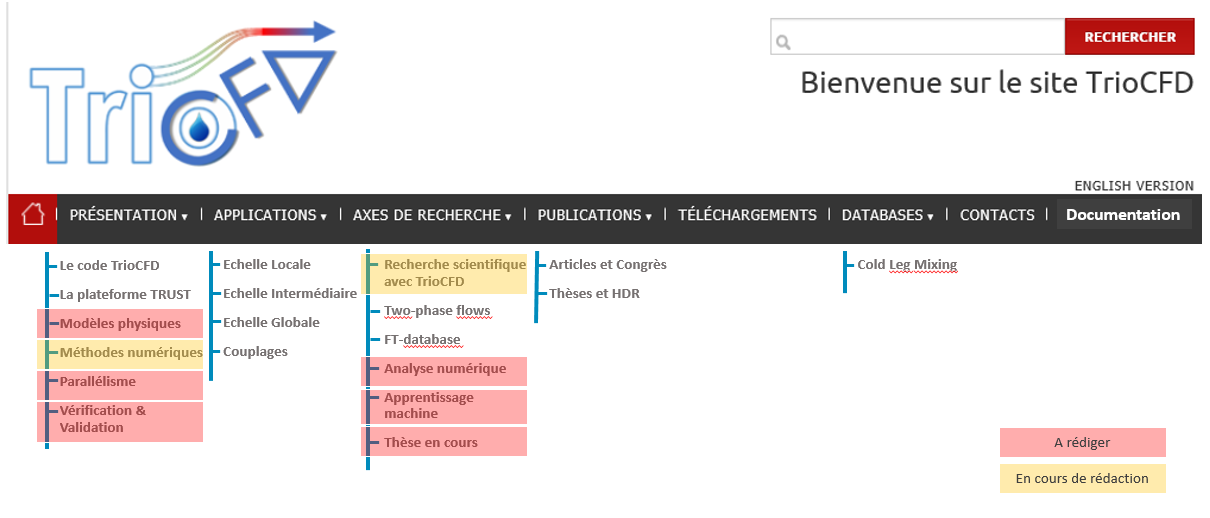
\includegraphics[width=14cm]{pictures/site_Trio.png}\end{center}
\begin{center}\captionof{figure}{\label{figure:structure_site_trio}Structure actuelle du site TrioCFD.}\end{center}

L'objectif du site est de pr\'esenter de fa\c con g\'en\'erale le code TrioCFD, les mod\`eles qui y sont impl\'ement\'es et les applicatifs pour lequel il est utilis\'e/applicable. Un bon nombre d'articles ou de rapport de th\`eses pr\'esentant les travaux effectu\'es avec TrioCFD y sont disponibles ainsi que la documentation du code (rapport de validation, documentation des mod\`eles, manuel de r\'ef\'erence). La page d'accueil regroupe les actualit\'es du code comme l'annonce de s\'eminaire, de sortie de version,... Le lien vers GitHub sur lequel le code source de TrioCFD est disponible est \'egalement r\'ef\'erenc\'e.\newline
Le site s'adresse autant aux utilisateurs interne CEA du code qu'aux utilisateurs universitaires ou industriels. Un formulaire de contact est à la disposition des utilisateurs (pour ceux ne connaissant pas l'adresse du projet) afin qu'ils soient n\'enamoins en mesure de prendre contact avec l'\'equipe en cas de question ou de problème.\newline\\
Pour l'instant, le site est tr\`es majoritairement en fran\c cais et toutes les parties nomm\'ees ci-dessus ne sont pas achev\'ees. Un travail de refonte du site est actuellement en cours afin notamment de l'enrichir avec les nouveaux applicatifs pour lesquels TrioCFD est utilis\'e. Lorsque le nouveau format du site sera termin\'e, celui-ci sera
exclusivement en anglais. Une premi\`ere maquette de la nouvelle structure du site est donn\'ee en figure \ref{figure:nouvelle_structure_site_trio}

\begin{center}
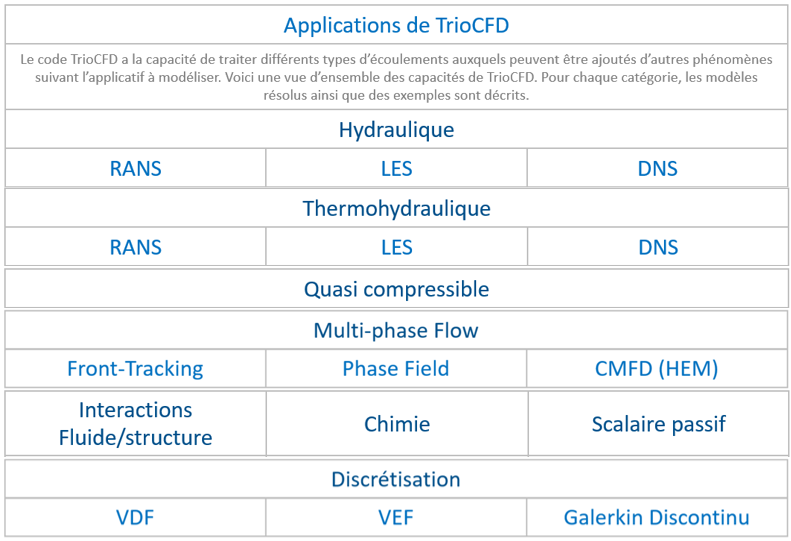
\includegraphics[width=10cm]{pictures/nouveau_site_trio.png}
\end{center}
\begin{center}
\captionof{figure}{\label{figure:nouvelle_structure_site_trio}$1^{\`ere}$ maquette de la nouvelle structure du site TrioCFD.}
\end{center}

Il s'agit l\`a d'une premi\`ere \'ebauche qui pourra \^etre quelque peu modifi\'ee lors de son impl\'ementation. Cette nouvelle structure a pour but de cr\'eer une cartographie compl\`ete et structur\'ee des domaines d'utilisation de TrioCFD, des mod\`eles utilis\'es pour chaque applicatif et des illustrations de ceux-ci par des exemples. Dans sa forme finale, le site pr\'esentera \'egalement l'\'equipe TrioCFD, le formulaire de contact sera conserv\'e ainsi que la base de donn\'ees (\texttt{DATABASE}) et les publications relatives \`a TrioCFD.

\chapter{GT et r\'eunion de d\'eveloppement}
\lhead{GT et r\'eunion de d\'eveloppement}
\rhead{COMMUNICATION}
Deux r\'eunions avec des formats diff\'erents ont lieu chaque mois :
\begin{itemize}[label=$\Rightarrow$, font=\LARGE]
\item \textbf{Groupe de Travail TrioCFD :} il s'agit d'une r\'eunion interne au laboratoire supportant TrioCFD, \`a savoir le LMSF, avec une orientation plut\^ot monophasique ; elle est anim\'ee par le chef de laboratoire. L'\'equipe fait un \'etat d'avancement sur les diff\'erentes t\^aches qui lui sont attribu\'ees sur TrioCFD. Les nouvelles collaborations sont \'egalement pr\'esent\'ees \`a l'ensemble de l'\'equipe avec les enjeux et les difficult\'es rencontr\'ees. Le chef de laboratoire communique \'egalement \`a l'ensemble de l'\'equipe les informations issues de la ligne hiérarchique, et le responsable de lot (SELMA) les informations issues de la ligne projet.
\item \textbf{R\'eunion de d\'eveloppement TrioCFD :} cette r\'eunion est ouverte \`a l'ensemble des utilisateurs et d\'eveloppeurs CEA de TrioCFD (quelque soit son laboratoire ou son site de rattachement) ; elle est anim\'ee par le responsable de code. Celui-ci \'evoque les sujets d'actualit\'e sur TrioCFD (sortie de version, d\'eveloppements en cours ou \`a venir, s\'eminaires,...). Il propose \'egalement \`a l'\'equipe, des outils et pratiques pour am\'eliorer la qualit\'e du code, les conditions de travail pour mener les \'etudes et les d\'eveloppements,... Apr\'es consensus sur ces outils et mise en place, leur utilisation est d\'etaill\'ee dans une r\'eunion de d\'eveloppement suivante.
\end{itemize}

Si un besoin particulier est exprim\'e, une r\'eunion suppl\'ementaire peut \^etre provoqu\'ee, ou la fr\'equence augment\'ee sur une p\'eriode donn\'ee.

\chapter{S\'eminaires}
\lhead{S\'eminaires}
\rhead{COMMUNICATION}

Diff\'erents formats de s\'eminaires rythment l'ann\'ee :
\begin{itemize}[label=$\Rightarrow$, font=\LARGE]
\item \textbf{S\'eminaire des \'etudiants :} Au d\'epart des stagiaires, doctorants ou post-doctorants, un s\'eminaire est organis\'e en interne CEA afin qu'ils pr\'esentent les travaux qui ont \'et\'e effectu\'es dans ce cadre. En ce qui concerne les stagiaires, le s\'eminaire regroupe plusieurs pr\'esentations traitant d'une m\^eme th\'ematique.
Ainsi, plusieurs s\'eminaires de ce type seront organis\'es chaque ann\'ee. Pour les doctorants, le s\'eminaire d\'edi\'e lui permet un entra\^inement en grandeur nature pour sa soutenance de th\`ese.
\item \textbf{S\'eminaire des permanents :} Lorsque un sujet de recherche, une \'etude ou un livrable est arriv\'e \`a maturit\'e, un s\'eminaire sp\'ecifique est organis\'e en interne CEA afin d'\'echanger sur le sujet.
\item \textbf{S\'eminaire TrioCFD :} Tous les 2 ans, le s\'eminaire TrioCFD est organis\'e avec l'ensemble des utilisateurs internes ou externes CEA. La journ\'ee s'articule autour de pr\'esentations techniques autant sur des applications pour lesquelles TrioCFD est utilis\'e pour la mod\'elisation que sur des d\'eveloppements majeurs de nouvelles fonctionnalit\'es. C'est une occasion pour les utilisateurs de d\'ecouvrir les avanc\'ees du code sur les deux derni\`eres ann\'ees et d'avoir un pannel complet des applicatifs. Une partie importante de la journ\'ee est \'egalement d\'edi\'ee aux \'echanges et au partage d'exp\'eriences.
\end{itemize}


